\section*{Metodolog\'ia}

\subsection*{1. Materiales}
\begin{itemize}
	\item Péndulo de Pohl PHYWE 11214-00
	\item Sensor-CASSY 2
	\item Fuente de poder PHYWE \qty{230}{\volt}, DC: 0...\qty{12}{\volt}, \qty{2}{\ampere}
	\item Multímetro digital
	\item Polea, anillo y cuerda ligera
	\item Computador
\end{itemize}

\subsection*{2. Esquema del Montaje}
\begin{figure}[H]
	\centering
	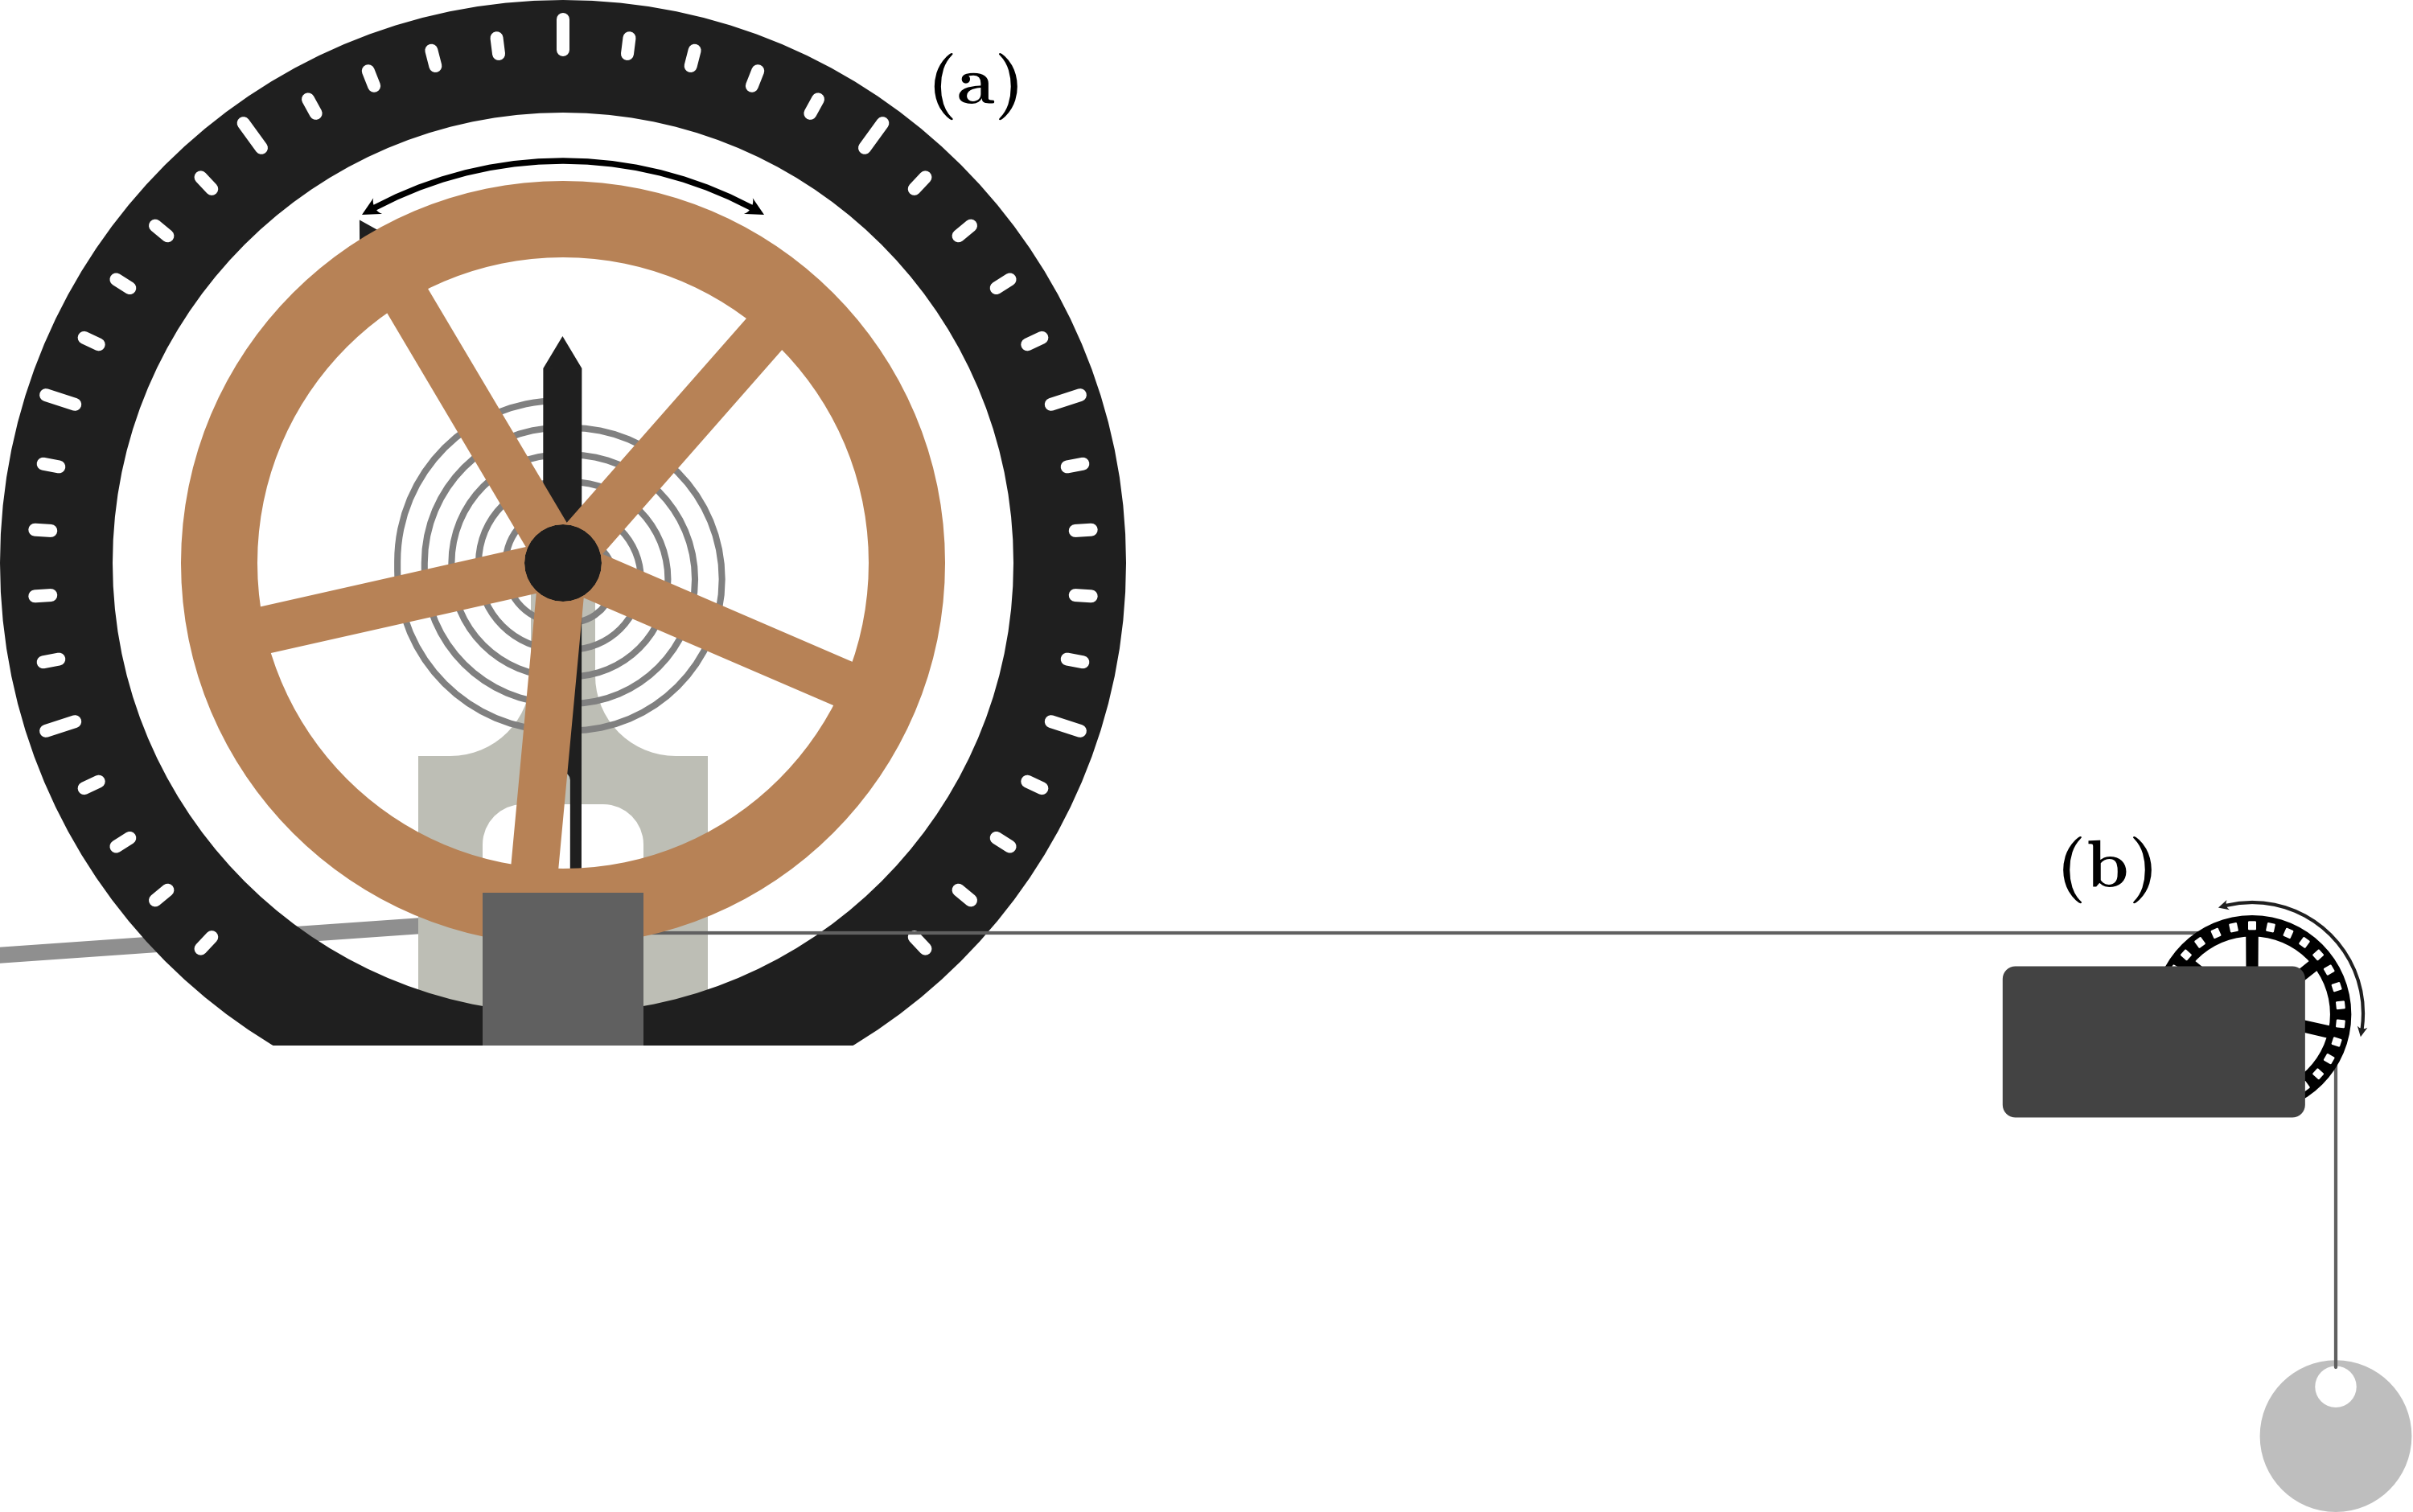
\includegraphics[width=\linewidth]{res/POHLFORZADO2.png}
	\captionof{figure}{Montaje experimental del péndulo de Pohl.
		\textbf{(a)} Péndulo de Pohl con una cuerda ligera sujetada al disco de cobre.
		La cuerda está amarrada a un anillo liviano para tensarla.
		\textbf{(b)} Polea ligera sosteniendo la cuerda. El sensor detecta la rotación
		de la polea permitiendo registrar la amplitud con respecto al tiempo.
	}
	\label{fig:montaje}
\end{figure}

\subsection*{3. Procedimiento}